\section{Testing the Seed-Selection Model}
\label{sec:seed-test-results}
To measure seed selection after the expanded training, we froze the
weights at the end of the twenty new passes and evaluated all
@TEST_TARGETS@ targets from @TEST_FAMILIES@ reserved families.
The test contains @SINGLE@ individual integrals and @EXPRESSION@
integral expressions, with loop orders from one through twelve.
It evaluates mass profiles excluded from parameter updates within
the family domains of Section~\ref{sec:integrals-generation}.
The fixed threshold remains $p_b=1/2$, and no test result changes
the weights or the confidence map~\cite{SeedModelTestData}.

\subsection{Reference agreement and seed ranking}
The test supplies @LABELS@ candidate labels, of which @POSITIVES@
belong to the recorded sufficient sets. A true positive is a
selected candidate with reference label one, while a false positive
is a selected candidate absent from that set. A false negative is
a recorded seed that the model omits. With these counts,
\begin{equation}
 {\rm precision}=\frac{\mathrm{TP}}{\mathrm{TP}+\mathrm{FP}},
 \qquad
 {\rm recall}=\frac{\mathrm{TP}}{\mathrm{TP}+\mathrm{FN}},
 \qquad
 F_1=\frac{2\,{\rm precision}\,{\rm recall}}
             {{\rm precision}+{\rm recall}} .
 \label{eq:seed-test-pr}
\end{equation}
The pooled precision is @PRECISION@\%, recall is @RECALL@\%
and $F_1$ is @F1@\%. The fraction of targets whose complete predicted
set equals its recorded set is @EXACT@\%. Candidate-label accuracy
is @ACCURACY@\%; the all-zero rule gives @ZERO_ACCURACY@\%
because zero labels are frequent. Precision, recall and complete-set
agreement therefore describe seed recovery more directly than
accuracy alone~\cite{SaitoRehmsmeier2015}.

\begin{figure}[htbp]
 \centering
 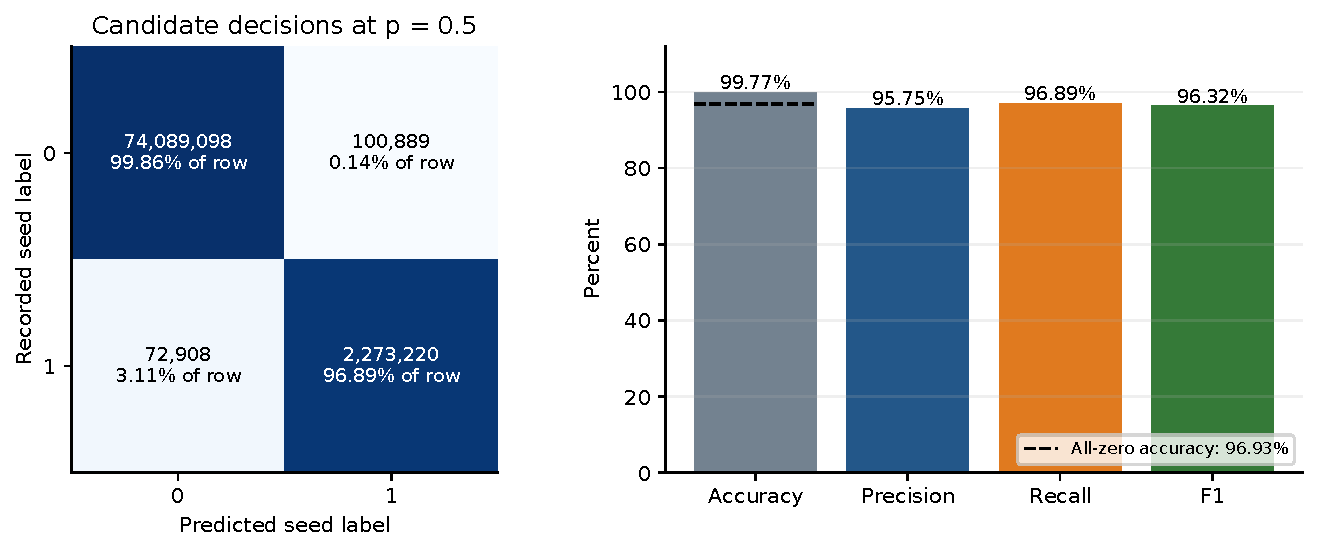
\includegraphics[width=\linewidth]{figures/seed_classification.pdf}
 \caption{Candidate decisions at the fixed threshold, with pooled
 precision, recall and $F_1$. Each confusion-matrix percentage is
 normalized within its reference-label row.}
 \label{fig:seed-classification}
\end{figure}

To examine the scores without changing the threshold, we rank
candidates by $p_b$ and group candidates with equal scores.
For a target $T$, let $P_g$ and $R_g$ be the precision and recall
after including score group $g$ in descending order. With $R_0=0$,
the target average precision is~\cite{AveragePrecisionDefinition}
\begin{equation}
 {\rm AP}_T=\sum_g (R_g-R_{g-1})P_g .
 \label{eq:seed-average-precision}
\end{equation}
Each increase in recovered reference seeds therefore weights the
precision at that point. Averaging over targets with at least one
recorded seed gives mean target average precision @MAP@\%.
The first ten candidates recover, on average, @RECALL10@\% of
recorded seeds and contain every recorded seed for @COVERAGE10@\%
of targets in the corresponding nonempty-reference comparison.
The score-curve calculation uses 4,096 fixed probability intervals;
it supplies a descriptive curve and does not select a new
operating threshold.

\begin{figure}[htbp]
 \centering
 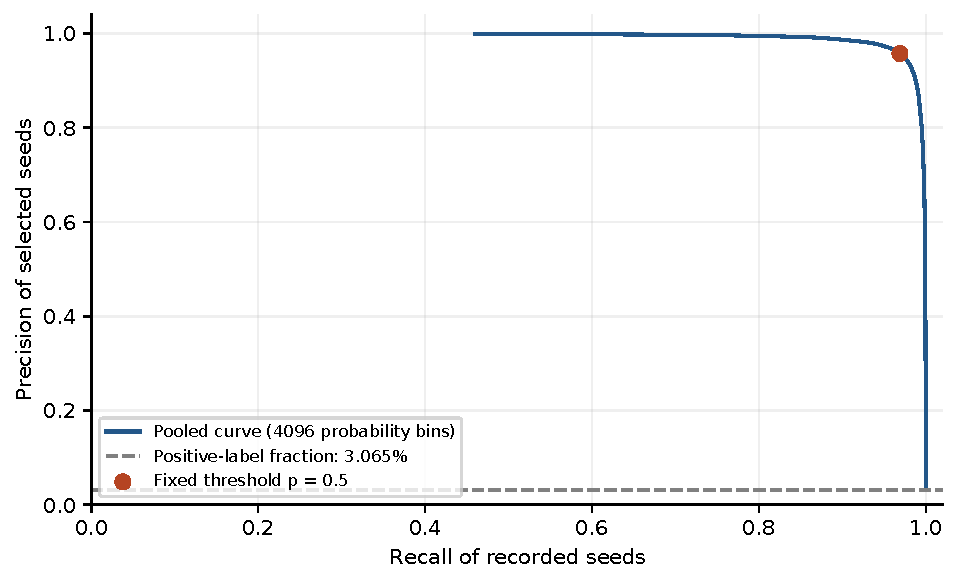
\includegraphics[width=0.80\linewidth]{figures/precision_recall.pdf}
 \caption{Pooled precision and recall as the score threshold varies.
 The marked point retains the fixed threshold of one half.
 The horizontal reference gives the positive-label fraction.}
 \label{fig:seed-precision-recall}
\end{figure}
\begin{figure}[htbp]
 \centering
 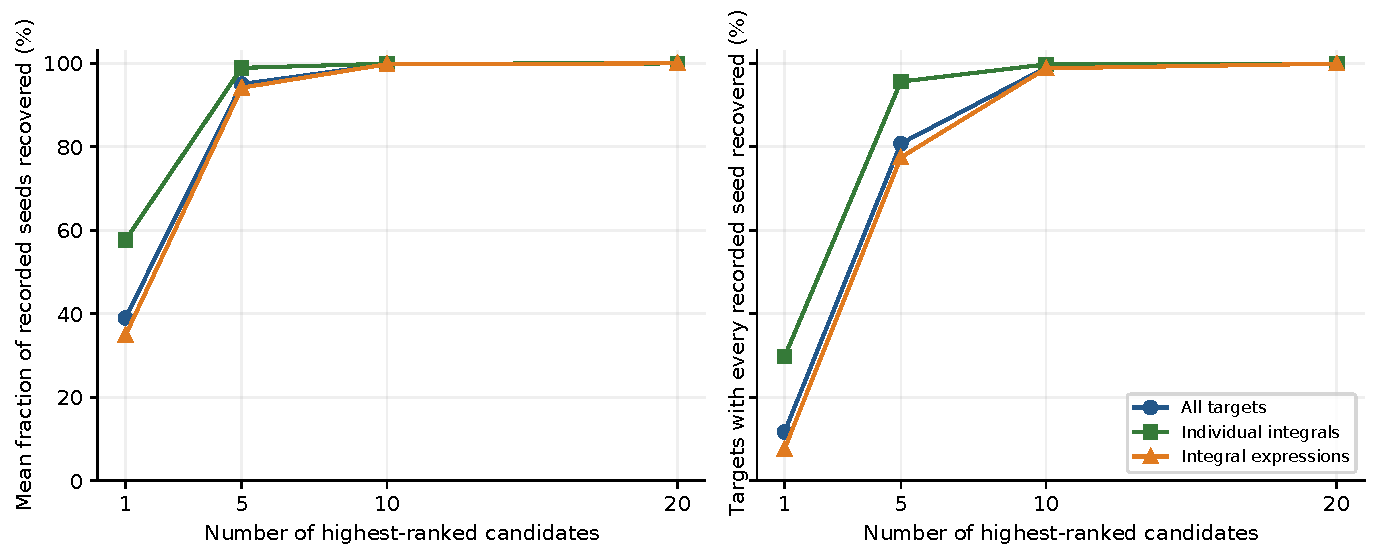
\includegraphics[width=\linewidth]{figures/ranked_seed_recovery.pdf}
 \caption{Recorded-seed recovery as the number of supplied
 highest-ranked candidates increases. The right panel requires every
 recorded seed to appear in the selected prefix. Individual
 integrals and integral expressions are also shown separately.}
 \label{fig:seed-ranking}
\end{figure}

\subsection{Confidence and dependence on the family}
For a returned binary label, the model reports $q_b$ from
Eq.~\eqref{eq:seed-binary-confidence}. We group decisions by this
value and compare their mean confidence with the fraction matching
the reference. Equality would place a group on the diagonal of
Figure~\ref{fig:seed-confidence}. These empirical comparisons assess
the saved scores without fitting a calibration correction.

\begin{figure}[htbp]
 \centering
 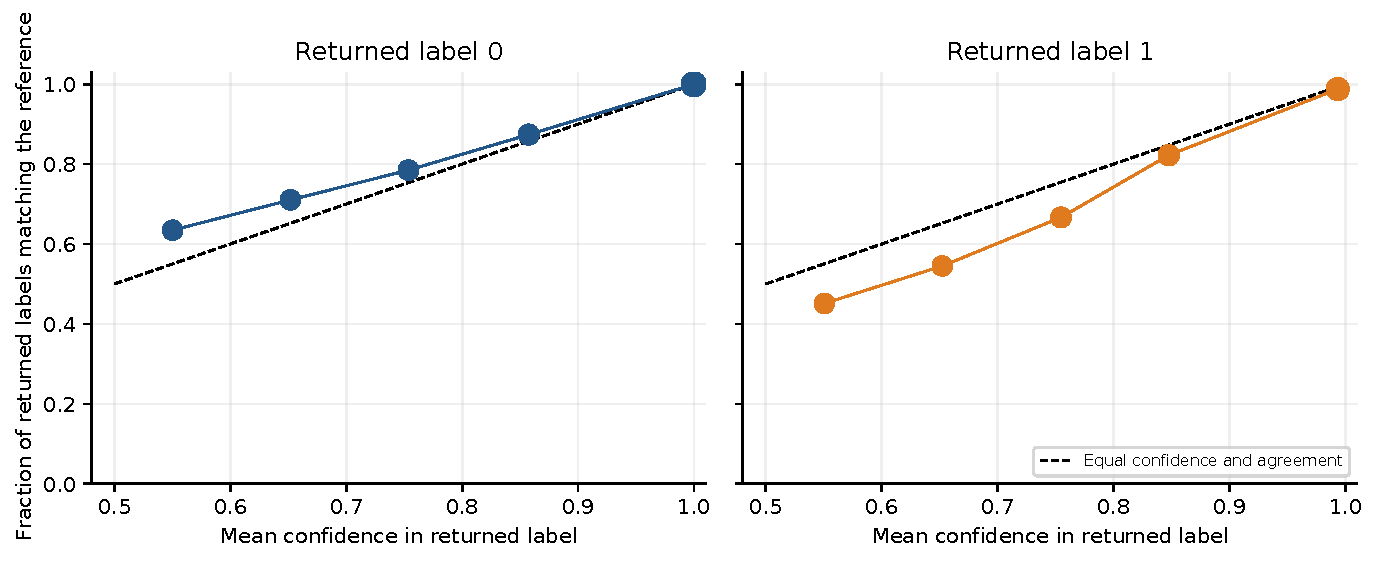
\includegraphics[width=\linewidth]{figures/confidence_calibration.pdf}
 \caption{Reported confidence and observed label agreement, shown
 separately for returned labels zero and one. Marker area increases
 with the number of decisions in a group.}
 \label{fig:seed-confidence}
\end{figure}

Figure~\ref{fig:seed-families} separates performance by family and
loop order. The one-loop group has @ONE_FAMILIES@ families,
the two-loop group has @TWO_FAMILIES@, and each remaining order
has 405 held-out mass profiles. This separation matters because
the added vacuum families use different identities and candidate
bounds from the earlier one-loop collection. Loop-order comparisons
also reflect these differences in the mathematical domain.
At one loop the pooled recall is @ONE_RECALL@\% and $F_1$ is
@ONE_F1@\%; at twelve loops they are @TWELVE_RECALL@\% and
@TWELVE_F1@\%, respectively. Across the groups from two through
twelve loops, the lowest recall is @MIN_HIGH_RECALL@\% at
$L=@MIN_HIGH_LOOP@$. These missed reference seeds show why a
proposed set still needs an exact sufficiency check before use in
a complete reduction.

\begin{figure}[htbp]
 \centering
 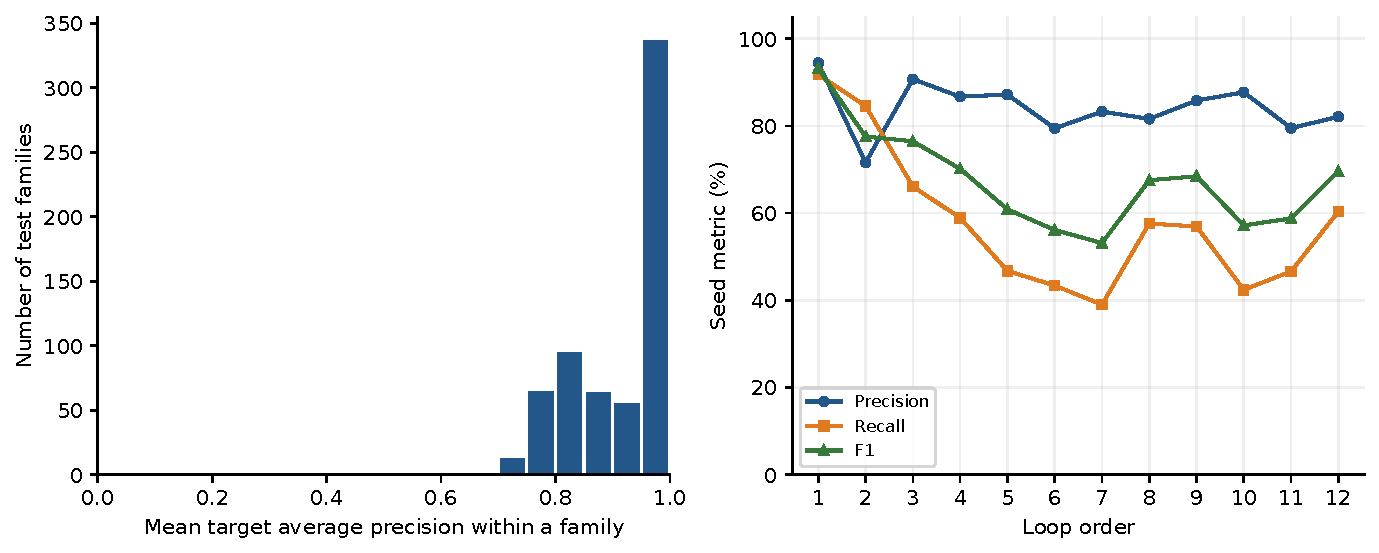
\includegraphics[width=\linewidth]{figures/family_performance.pdf}
 \caption{Distribution of mean target average precision across
 held-out families, and pooled seed precision, recall and $F_1$ at
 each loop order. The higher-loop groups cover the restricted
 vacuum mass profiles defined in the text.}
 \label{fig:seed-families}
\end{figure}

\subsection{Checks and interpretation}
Independent checks reproduce the saved confusion counts and target
counts, verify the prediction hashes and confirm that the weights
remain fixed. All stored probabilities are finite and lie between
zero and one. The mean time for input preparation and model
inference is @INFERENCE_MS@ ms per target on the test allocation;
this excludes a subsequent exact reduction.

The labels identify one recorded sufficient set. Other seed sets can
also reduce the target, so disagreement with these labels does not
by itself establish failure of the proposed reduction. This test
measures reference-set recovery and confidence. It does not run
Kira with the predicted seed sets, prove seed minimality or measure
a solver speedup. The next model addresses the separate choice of
an allowed elimination step after equations are available.
\FloatBarrier
